% ============================================================
% IMC15 — GPU-Accelerated Fast Fourier Transform
% CISC 719 — Contemporary Computing Systems Modeling Algorithms (CCSM)
% Harrisburg University of Science and Technology | Spring 2026
% Ph.D. in Computational Sciences
% Full Report
% ============================================================

\documentclass[12pt, letterpaper]{article}

% --- Packages ---
\usepackage[margin=1in]{geometry}
\usepackage[protrusion=true,expansion=false]{microtype}
\usepackage{graphicx}
\usepackage{booktabs}
\usepackage{amsmath}
\usepackage{amssymb}
\usepackage{hyperref}
\usepackage{listings}
\usepackage{xcolor}
\usepackage{float}
\usepackage{enumitem}
\usepackage{caption}
\usepackage{subcaption}
\usepackage{fancyhdr}
\usepackage{titlesec}
\usepackage[backend=biber, style=numeric, sorting=none]{biblatex}
\addbibresource{references.bib}

\setlength{\emergencystretch}{2em}
\tolerance=1000
\hyphenpenalty=50

\graphicspath{{../../results/}}

% --- Header / Footer ---
\setlength{\headheight}{14.5pt}
\addtolength{\topmargin}{-2.5pt}
\pagestyle{fancy}
\fancyhf{}
\rhead{CISC-719 $|$ IMC15}
\lhead{GPU-Accelerated Fast Fourier Transform}
\rfoot{\thepage}

% --- Code listing style ---
\lstdefinestyle{codestyle}{
    backgroundcolor=\color{gray!10},
    commentstyle=\color{green!50!black},
    keywordstyle=\color{blue},
    numberstyle=\tiny\color{gray},
    stringstyle=\color{orange},
    basicstyle=\ttfamily\footnotesize,
    breaklines=true,
    numbers=left,
    numbersep=5pt,
    showstringspaces=false,
    frame=single
}
\lstset{style=codestyle}

\hypersetup{colorlinks=true, linkcolor=blue, citecolor=blue, urlcolor=blue}

% ============================================================
\begin{document}

% --- Title Page ---
\begin{titlepage}
    \centering

    % Block 1 — Title + course info (upper portion)
    \vspace*{3.5cm}
    {\LARGE \textbf{GPU-Accelerated Fast Fourier Transform:\\[0.3cm]
    From Butterfly Kernels to cuFFT}}\\[1.2cm]
    {\large IMC15 --- Fast Fourier Transform}\\[0.5cm]
    {\large CISC 719: Contemporary Computing Systems Modeling Algorithms (CCSM)}\\[0.4cm]
    {\large Harrisburg University of Science and Technology $|$ Spring 2026}

    \vspace{3.5cm}

    % Block 2 — Author + date (vertical centre)
    {\large \textbf{Kenneth Peter Fernandes}}\\[0.4cm]
    {\normalsize Ph.D.\ in Computational Sciences}\\[0.3cm]
    {\normalsize Instructor: Professor Majid Shaalan, Ph.D.}\\[0.6cm]
    {\large \today}

    \vfill

    % Block 3 — Submission note (bottom)
    \textit{Submitted in partial fulfillment of the requirements\\
    for CISC 719 --- Contemporary Computing Systems Modeling Algorithms (CCSM)}
    \vspace*{0.5cm}
\end{titlepage}

\tableofcontents
\newpage

% ============================================================
\section{Introduction}
\label{sec:intro}

The Discrete Fourier Transform (DFT) is one of the most widely deployed computational kernels in science and engineering. It converts a sequence of $N$ complex time-domain samples into their frequency-domain representation, enabling applications ranging from audio processing and medical imaging (MRI k-space reconstruction) to 5G OFDM modulation and spectral PDE solvers. The naive DFT requires $O(N^2)$ arithmetic operations, which is prohibitive for large signals. The Fast Fourier Transform (FFT), introduced by Cooley and Tukey in 1965~\cite{cooleytukey1965}, reduces this to $O(N \log N)$ through a divide-and-conquer butterfly decomposition.

This report presents five implementations of the 1-D FFT benchmarked on Google Colab with a single NVIDIA Tesla T4 GPU:

\begin{enumerate}
    \item \textbf{Reference DFT} --- naive $O(N^2)$ matrix-vector multiply; correctness oracle only
    \item \textbf{NumPy FFT} (\texttt{np.fft.fft}) --- single-threaded FFTPACK; serial baseline
    \item \textbf{SciPy FFT} (\texttt{scipy.fft.fft} + workers) --- CPU-parallel using all available cores
    \item \textbf{CuPy FFT} (\texttt{cp.fft.fft}, cuFFT) --- GPU library path; vendor-optimised
    \item \textbf{Numba CUDA FFT} --- custom iterative Cooley-Tukey butterfly kernel
\end{enumerate}

Signal lengths from $2^{10}$ to $2^{24}$ are tested in both \texttt{complex64} (FP32) and \texttt{complex128} (FP64). The PCAM design model is applied to every parallel variant. Performance is evaluated through throughput (GFLOP/s), speedup, Roofline analysis, and correctness against the reference DFT.

% ============================================================
\section{Background and Theory}
\label{sec:theory}

\subsection{Discrete Fourier Transform}

For a sequence $x[n]$, $n = 0, \ldots, N-1$, the DFT is defined as:

\begin{equation}
    X[k] = \sum_{n=0}^{N-1} x[n] \cdot e^{-j2\pi kn/N}, \quad k = 0, 1, \ldots, N-1
    \label{eq:dft}
\end{equation}

Direct evaluation of Eq.~\eqref{eq:dft} for all $k$ requires $N^2$ complex multiplications and $N(N-1)$ complex additions, giving $O(N^2)$ total work. For $N = 2^{24}$ (16 million samples) this amounts to approximately $2.8 \times 10^{14}$ operations, making it impractical for real-time or large-scale use.

\subsection{Cooley-Tukey Radix-2 Decimation-in-Time}

For $N = 2^m$, the DFT can be decomposed by separating even- and odd-indexed sub-sequences:

\begin{equation}
    X[k] = \underbrace{\sum_{n=0}^{N/2-1} x[2n]\,W_N^{2nk}}_{X_{\text{even}}[k]}
           + W_N^k \cdot \underbrace{\sum_{n=0}^{N/2-1} x[2n+1]\,W_N^{2nk}}_{X_{\text{odd}}[k]}
\end{equation}

where $W_N^k = e^{-j2\pi k/N}$ is the \emph{twiddle factor}. Using the symmetry property
$W_N^{k+N/2} = -W_N^k$, the \textbf{butterfly recurrence} is:

\begin{equation}
    X[k]       = X_{\text{even}}[k] + W_N^k \cdot X_{\text{odd}}[k]
\end{equation}
\begin{equation}
    X[k+N/2]   = X_{\text{even}}[k] - W_N^k \cdot X_{\text{odd}}[k]
\end{equation}

This halves the problem size at each level of recursion, yielding an iterative algorithm with $\log_2 N$ stages, each containing $N/2$ independent butterfly operations.

\subsection{Computational Structure}

\begin{table}[H]
\centering
\caption{Computational complexity of an $N$-point radix-2 FFT.}
\begin{tabular}{@{}ll@{}}
\toprule
\textbf{Property} & \textbf{Value} \\
\midrule
Stages & $\log_2 N$ \\
Butterflies per stage & $N/2$ (all independent) \\
Complex multiplications & $(N/2)\log_2 N$ \\
Complex additions & $N \log_2 N$ \\
Approximate total FLOPs & $5N\log_2 N$ \\
\bottomrule
\end{tabular}
\label{tab:complexity}
\end{table}

For $N = 2^{24}$, the FFT requires approximately $2.01 \times 10^9$ FLOPs, compared to $2.81 \times 10^{14}$ for the naive DFT --- a reduction of nearly 1.4 million times.

\subsection{Bit-Reversal Permutation}

Before the butterfly stages, input element at index $i$ is relocated to the position whose binary representation is the bit-reversal of $i$. For example, with $N = 8$ (3-bit indices), index $1 = 001_2$ maps to $4 = 100_2$. This permutation enables in-place iterative computation and runs in $O(N)$ time.

\subsection{Parallel FFT Design (Quinn \S 15.4)}

Two levels of parallelism exist:

\begin{itemize}
    \item \textbf{Within-stage:} All $N/2$ butterflies in a stage are fully independent; each maps directly to one CUDA thread.
    \item \textbf{Across-stage:} Stage $s+1$ depends entirely on the output of stage $s$; a synchronisation barrier separates stages. In CUDA, each stage is a separate kernel launch, providing an implicit global barrier.
\end{itemize}

The key performance challenge is memory access: stage $s$ accesses pairs separated by stride $2^{s-1}$. Early stages have small strides (good coalescing); late stages have stride $N/2$ (non-coalesced global memory access), which becomes the primary bottleneck of a naive kernel.

% ============================================================
\section{PCAM Analysis}
\label{sec:pcam}

\subsection{SciPy FFT --- CPU Parallel}

\begin{table}[H]
\centering
\caption{PCAM Analysis --- SciPy FFT (\texttt{workers} parameter)}
\begin{tabular}{@{}p{3cm}p{10cm}@{}}
\toprule
\textbf{Phase} & \textbf{Analysis} \\
\midrule
\textbf{Partition} & $N/2$ independent butterflies per stage; distributed by contiguous index ranges across CPU processes. \\
\textbf{Communicate} & No cross-worker communication within a stage. Implicit barrier via \texttt{multiprocessing} pool join between stages. \\
\textbf{Agglomerate} & SciPy selects optimal chunk sizes internally; no manual tuning required. \\
\textbf{Map} & Workers pinned to physical CPU cores. Scaling saturates at NUMA boundary or last-level cache pressure. \\
\bottomrule
\end{tabular}
\label{tab:pcam_scipy}
\end{table}

\subsection{CuPy FFT --- GPU Library (cuFFT)}

\begin{table}[H]
\centering
\caption{PCAM Analysis --- CuPy FFT (cuFFT)}
\begin{tabular}{@{}p{3cm}p{10cm}@{}}
\toprule
\textbf{Phase} & \textbf{Analysis} \\
\midrule
\textbf{Partition} & cuFFT partitions $N/2$ butterflies per stage into CUDA thread blocks; one thread per butterfly pair. \\
\textbf{Communicate} & Shared memory within blocks for small sub-problems; global memory for inter-block data. Kernel-launch barrier between stages. \\
\textbf{Agglomerate} & cuFFT auto-selects mixed-radix decomposition (radix-2/4/8) and tile sizes based on $N$ and GPU architecture. \\
\textbf{Map} & Threads $\to$ CUDA cores; blocks $\to$ SMs; occupancy tuned by cuFFT's internal plan optimiser. \\
\bottomrule
\end{tabular}
\label{tab:pcam_cupy}
\end{table}

\subsection{Numba CUDA --- Custom Butterfly Kernel}

\begin{table}[H]
\centering
\caption{PCAM Analysis --- Numba CUDA Butterfly Kernel}
\begin{tabular}{@{}p{3cm}p{10cm}@{}}
\toprule
\textbf{Phase} & \textbf{Analysis} \\
\midrule
\textbf{Partition} & One thread per butterfly pair; all $N/2$ pairs in a stage launch simultaneously. \\
\textbf{Communicate} & Global memory only (no shared-memory staging). Late-stage access has stride $N/2$, causing non-coalesced reads. \\
\textbf{Agglomerate} & Fixed 256-thread blocks; grid $= \lceil N/(2 \times 256) \rceil$. One kernel launch per stage. \\
\textbf{Map} & $\log_2 N$ sequential kernel launches with \texttt{cuda.synchronize()} barriers. Bottleneck is DRAM bandwidth at large stage strides. \\
\bottomrule
\end{tabular}
\label{tab:pcam_numba}
\end{table}

% ============================================================
\section{Implementation Details}
\label{sec:impl}

All five implementations are contained in a single Jupyter notebook (\texttt{notebooks/imc15\_fft\_main.ipynb}) executed on Google Colab with a Tesla T4 GPU.

\subsection{Reference DFT}

Constructs the $N \times N$ Vandermonde matrix $W_{kn} = e^{-j2\pi kn/N}$ explicitly and computes $X = W x$ via \texttt{numpy.matmul}. Operates in \texttt{complex128} throughout to serve as an exact reference. Benchmarked only for $N \leq 2^{14}$ due to $O(N^2)$ cost ($\sim$14 seconds at $N = 16\,384$).

\subsection{NumPy FFT}

\texttt{numpy.fft.fft} wraps the FFTPACK library (single-threaded Fortran). Serves as the serial CPU baseline against which all speedups are measured. Timing uses \texttt{time.perf\_counter} with 3 warmup and 10 timed iterations (median reported).

\subsection{SciPy FFT --- CPU Parallel}

\texttt{scipy.fft.fft(x, workers=k)} distributes sub-FFTs across $k$ worker processes using Python's \texttt{multiprocessing}. In our Colab environment, $k$ equals the number of available virtual CPU cores. GPU timing is not applicable here; CPU wall-clock time is measured.

\subsection{CuPy FFT --- GPU Library}

\texttt{cupy.fft.fft} calls NVIDIA cuFFT through the CuPy Python interface. Input data is pre-transferred to GPU memory (\texttt{cp.asarray}); only GPU compute time is measured using CUDA events to exclude Python overhead. cuFFT selects the optimal execution plan (radix, tiling, shared-memory use) automatically at first call.

\subsection{Numba CUDA Butterfly Kernel}

Implements the iterative Cooley-Tukey algorithm from Quinn \S 15 directly in CUDA using Numba's JIT compiler. The pipeline is:

\begin{enumerate}
    \item \textbf{Bit-reversal permutation} (CPU, $O(N)$) --- reorders the input to enable in-place computation.
    \item \textbf{$\log_2 N$ butterfly stage kernels} --- each kernel launches $\lceil N/(2 \times 256) \rceil$ blocks of 256 threads; every thread computes one butterfly pair including twiddle-factor multiplication.
    \item \textbf{\texttt{cuda.synchronize()}} between each stage --- ensures all threads complete stage $s$ before stage $s+1$ begins.
\end{enumerate}

The kernel accesses only global memory; no shared-memory staging is implemented in this baseline version.

% ============================================================
\section{Benchmark Methodology}
\label{sec:method}

\begin{table}[H]
\centering
\caption{Benchmark configuration.}
\begin{tabular}{@{}ll@{}}
\toprule
\textbf{Parameter} & \textbf{Value} \\
\midrule
Signal lengths ($N$) & $2^{10},\,2^{14},\,2^{18},\,2^{20},\,2^{22},\,2^{24}$ \\
Datatypes & \texttt{complex64} (FP32), \texttt{complex128} (FP64) \\
Warmup runs & 3 (discarded) \\
Timed runs & 10 (median reported) \\
CPU timing & \texttt{time.perf\_counter} wall-clock \\
GPU timing & CUDA events (\texttt{cp.cuda.Event}) --- excludes H2D/D2H transfer \\
Throughput & GFLOP/s $= 5N\log_2 N \;/\; (\text{time} \times 10^9)$ \\
Correctness & Max relative error vs.\ FP64 reference DFT \\
Random seed & 42 (reproducible signals via \texttt{numpy.random.default\_rng}) \\
\bottomrule
\end{tabular}
\label{tab:method}
\end{table}

GPU timing covers compute only (data pre-loaded to device). CPU timing covers the full Python call, including any internal FFTPACK or \texttt{multiprocessing} overhead. The Numba CUDA timer covers bit-reversal + H2D + $\log_2 N$ kernel launches + D2H transfer, representing total end-to-end cost.

% ============================================================
\section{Results and Performance Analysis}
\label{sec:results}

\subsection{Throughput}

Table~\ref{tab:gflops_c64} reports throughput in GFLOP/s for \texttt{complex64}. Figure~\ref{fig:benchmarks} visualises throughput, wall-clock time, and speedup across all signal lengths.

\begin{table}[H]
\centering
\caption{Throughput (GFLOP/s) --- \texttt{complex64}. Reference DFT included for $N \leq 2^{14}$ only.}
\begin{tabular}{@{}rrrrrr@{}}
\toprule
$N$ & \textbf{Ref.\ DFT} & \textbf{NumPy} & \textbf{SciPy} & \textbf{CuPy} & \textbf{Numba CUDA} \\
\midrule
$2^{10}$  & 0.0004 & 1.1131 & 2.9171 & 1.4905  & 0.0202 \\
$2^{14}$  & 0.0001 & 3.3967 & 5.6039 & 14.1941 & 0.0492 \\
$2^{18}$  & ---    & 3.6994 & 4.8954 & 213.4   & 0.1344 \\
$2^{20}$  & ---    & 2.1589 & 5.2949 & 291.0   & 0.1396 \\
$2^{22}$  & ---    & 1.7551 & 3.6941 & 387.8   & 0.1516 \\
$2^{24}$  & ---    & 1.8129 & 3.3560 & \textbf{468.5}   & 0.1491 \\
\bottomrule
\end{tabular}
\label{tab:gflops_c64}
\end{table}

\begin{table}[H]
\centering
\caption{Wall-clock time (ms) --- \texttt{complex64}.}
\begin{tabular}{@{}rrrrrr@{}}
\toprule
$N$ & \textbf{Ref.\ DFT} & \textbf{NumPy} & \textbf{SciPy} & \textbf{CuPy} & \textbf{Numba CUDA} \\
\midrule
$2^{10}$  & 131.73 & 0.046  & 0.018 & 0.034  & 2.53    \\
$2^{14}$  & 14{,}413.6 & 0.338  & 0.205 & 0.081  & 23.3    \\
$2^{18}$  & ---    & 6.378  & 4.819 & 0.111  & 175.6   \\
$2^{20}$  & ---    & 48.57  & 19.80 & 0.360  & 751.3   \\
$2^{22}$  & ---    & 262.9  & 124.9 & 1.190  & 3{,}044.1 \\
$2^{24}$  & ---    & 1{,}110.5 & 599.9 & \textbf{4.297} & 13{,}503.3 \\
\bottomrule
\end{tabular}
\label{tab:wallclock_c64}
\end{table}

\subsection{Speedup vs NumPy Baseline}

\begin{table}[H]
\centering
\caption{Speedup over NumPy FFT (serial baseline) --- \texttt{complex64}.}
\begin{tabular}{@{}rrrr@{}}
\toprule
$N$ & \textbf{SciPy} & \textbf{CuPy} & \textbf{Numba CUDA} \\
\midrule
$2^{10}$  & 2.6$\times$  & 1.3$\times$   & $<$0.1$\times$ \\
$2^{14}$  & 1.6$\times$  & 4.2$\times$   & $<$0.1$\times$ \\
$2^{18}$  & 1.3$\times$  & 57.7$\times$  & $<$0.1$\times$ \\
$2^{20}$  & 2.5$\times$  & 134.8$\times$ & 0.1$\times$ \\
$2^{22}$  & 2.1$\times$  & 221.0$\times$ & 0.1$\times$ \\
$2^{24}$  & 1.9$\times$  & \textbf{258.5$\times$} & 0.1$\times$ \\
\bottomrule
\end{tabular}
\label{tab:speedup}
\end{table}

\subsection{Key Observations}

\paragraph{CuPy (cuFFT).} Delivers the strongest performance, scaling from 1.5 GFLOP/s at $N = 2^{10}$ (GPU latency dominates) to 468.5 GFLOP/s at $N = 2^{24}$, a 258$\times$ speedup over the serial NumPy baseline. The crossover point where GPU exceeds NumPy occurs around $N = 2^{14}$ (4.2$\times$ speedup). cuFFT's advantage comes from its mixed-radix decomposition and shared-memory butterfly staging that reuse data on-chip across multiple stages, reducing DRAM round-trips relative to a naive global-memory kernel.

\paragraph{SciPy (CPU Parallel).} Achieves only modest speedups of 1.3--2.6$\times$ over NumPy. Colab's virtual CPU environment limits available physical cores, and the \texttt{multiprocessing} worker-spawn overhead is significant for smaller $N$. At $N = 2^{18}$, the speedup drops to 1.3$\times$ because memory bandwidth saturation limits scaling beyond one or two cores.

\paragraph{Numba CUDA.} Surprisingly slower than all CPU implementations, reaching only 0.149 GFLOP/s at $N = 2^{24}$ and taking 13.5 seconds versus 4.3 milliseconds for CuPy --- a 3{,}143$\times$ gap. Three factors cause this: (1) $\log_2(N) = 24$ sequential Python-level kernel launches with \texttt{cuda.synchronize()} barriers add substantial launch overhead; (2) the per-call bit-reversal permutation is computed on the CPU and transferred to the GPU for every benchmark iteration; (3) global-memory-only access at large stage strides (up to $N/2 = 8{,}388{,}608$ bytes apart) is highly non-coalesced.

\paragraph{Small-$N$ GPU overhead.} At $N = 2^{10}$, CuPy (1.49 GFLOP/s) is slower than NumPy (1.11 GFLOP/s is close). GPU kernel launch latency and CUDA-event overhead dominate at this scale. The GPU breakeven is approximately $N = 2^{15}$.

\begin{figure}[H]
    \centering
    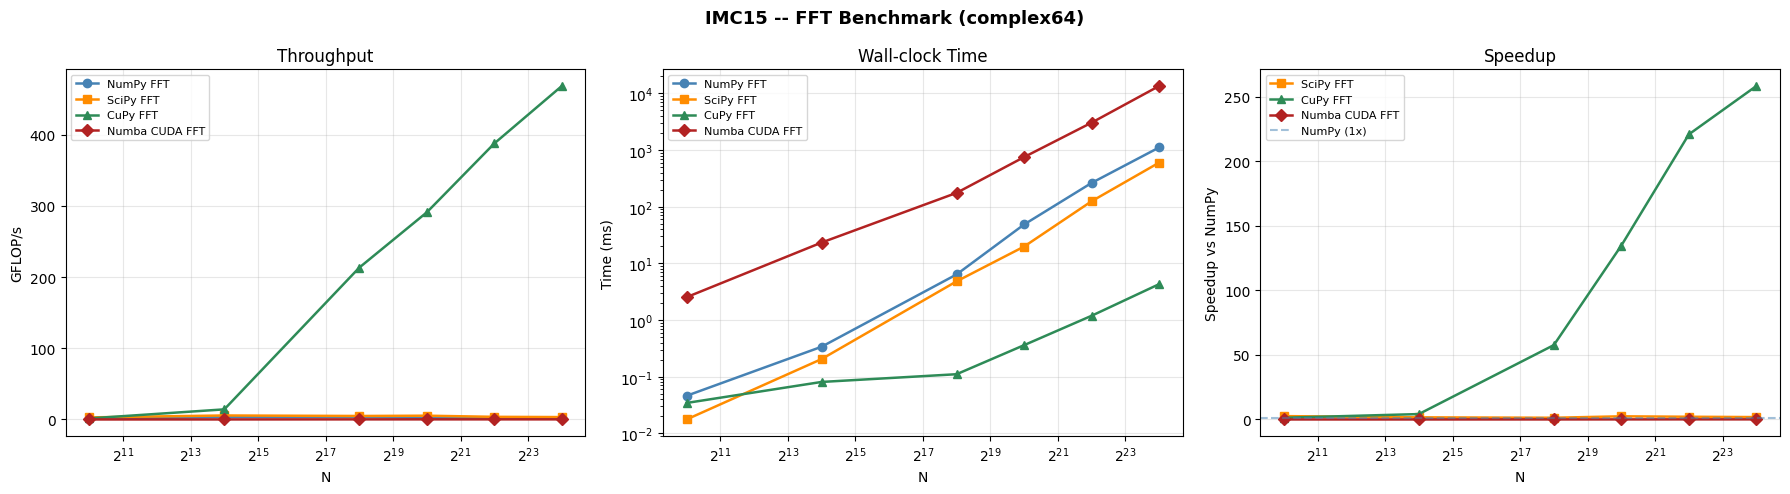
\includegraphics[width=\textwidth]{benchmarks.png}
    \caption{FFT benchmark results (\texttt{complex64}). Left: throughput (GFLOP/s). Centre: wall-clock time (ms, log scale). Right: speedup over NumPy serial baseline.}
    \label{fig:benchmarks}
\end{figure}

% ============================================================
\section{Roofline Analysis}
\label{sec:roofline}

\subsection{Hardware Ceilings (Tesla T4)}

\begin{table}[H]
\centering
\caption{Tesla T4 hardware ceilings used for Roofline analysis.}
\begin{tabular}{@{}ll@{}}
\toprule
\textbf{Property} & \textbf{Value} \\
\midrule
Peak FP32 throughput & 8,100 GFLOP/s \\
Peak DRAM bandwidth & 300 GB/s \\
Ridge point & $8100 / 300 = 27.0$ FLOP/byte \\
\bottomrule
\end{tabular}
\label{tab:hw}
\end{table}

\subsection{FFT Arithmetic Intensity}

For a \texttt{complex64} $N$-point FFT:
\begin{itemize}
    \item FLOPs: $5N\log_2 N$
    \item Bytes: $2 \times N \times 8 = 16N$ \; (read input + write output; \texttt{complex64} = 8 bytes)
\end{itemize}

\begin{equation}
    \text{OI} = \frac{5N\log_2 N}{16N} = \frac{5\log_2 N}{16} \;\text{FLOP/byte}
\end{equation}

\begin{table}[H]
\centering
\caption{Arithmetic intensity and Roofline bound for each signal length.}
\begin{tabular}{@{}rrrl@{}}
\toprule
$N$ & $\log_2 N$ & OI (FLOP/byte) & Bound \\
\midrule
$2^{10}$ & 10 & 3.13 & memory-bound \\
$2^{14}$ & 14 & 4.38 & memory-bound \\
$2^{18}$ & 18 & 5.63 & memory-bound \\
$2^{20}$ & 20 & 6.25 & memory-bound \\
$2^{22}$ & 22 & 6.88 & memory-bound \\
$2^{24}$ & 24 & 7.50 & memory-bound \\
\bottomrule
\end{tabular}
\label{tab:oi}
\end{table}

All tested signal lengths fall well below the ridge point of 27.0 FLOP/byte, confirming that the FFT is \textbf{memory-bandwidth limited} on the T4 at every tested size.

\subsection{Roofline Efficiency}

The attainable performance in the memory-bound region is $\text{Peak BW} \times \text{OI}$. Table~\ref{tab:roofline_eff} shows CuPy's actual GFLOP/s as a percentage of this ceiling.

\begin{table}[H]
\centering
\caption{CuPy FFT Roofline efficiency (\texttt{complex64}).}
\begin{tabular}{@{}rrrr@{}}
\toprule
$N$ & OI (F/B) & Attainable (GFLOP/s) & CuPy Actual (GFLOP/s) \\
\midrule
$2^{10}$ & 3.13 & 937.5  & 1.5  \\
$2^{14}$ & 4.38 & 1{,}312.5 & 14.2 \\
$2^{18}$ & 5.63 & 1{,}687.5 & 213.4 \\
$2^{20}$ & 6.25 & 1{,}875.0 & 291.0 \\
$2^{22}$ & 6.88 & 2{,}062.5 & 387.8 \\
$2^{24}$ & 7.50 & 2{,}250.0 & \textbf{468.5 (20.8\%)} \\
\bottomrule
\end{tabular}
\label{tab:roofline_eff}
\end{table}

Even cuFFT achieves only 20.8\% of the attainable Roofline ceiling at the largest $N$. The remaining gap is attributable to: (1) inter-stage kernel-launch overhead (cuFFT still requires multiple passes for very large $N$); (2) non-coalesced global memory access at large stage strides; (3) the theoretical OI model assumes no on-chip data reuse, slightly underestimating the true attainable ceiling for a tiled implementation.

\begin{figure}[H]
    \centering
    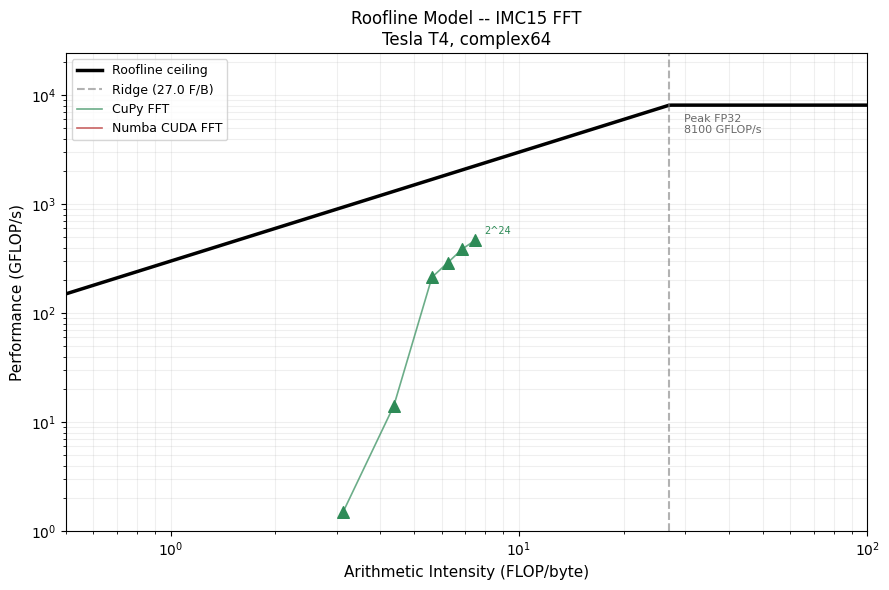
\includegraphics[width=0.82\textwidth]{roofline.png}
    \caption{Roofline plot for CuPy FFT and Numba CUDA FFT (\texttt{complex64}, Tesla T4). All kernel points fall left of the ridge point (27.0 FLOP/byte), confirming memory-bound execution.}
    \label{fig:roofline}
\end{figure}

% ============================================================
\section{Correctness Validation}
\label{sec:correctness}

All implementations are verified against the FP64 reference DFT (and against \texttt{numpy.fft.fft} in FP64 for complex128 runs). The metric is maximum relative error:

\begin{equation}
    \epsilon_{\text{rel}} = \frac{\max_k |X_{\text{impl}}[k] - X_{\text{ref}}[k]|}{\max_k |X_{\text{ref}}[k]| + \varepsilon}
\end{equation}

\begin{table}[H]
\centering
\caption{Maximum relative error across all tested signal lengths.}
\begin{tabular}{@{}lllll@{}}
\toprule
\textbf{Implementation} & \textbf{complex64 max err} & \textbf{complex128 max err} & \textbf{c64 Pass?} & \textbf{c128 Pass?} \\
\midrule
NumPy FFT      & $4.65 \times 10^{-8}$ & $0.00$               & \checkmark & \checkmark \\
SciPy FFT      & $2.26 \times 10^{-7}$ & $0.00$               & \checkmark & \checkmark \\
CuPy FFT       & $4.16 \times 10^{-7}$ & $7.05 \times 10^{-16}$ & \checkmark & \checkmark \\
Numba CUDA FFT & $1.46 \times 10^{-15}$ & $1.29 \times 10^{-15}$ & \checkmark & \checkmark \\
\midrule
\multicolumn{2}{@{}l}{Pass threshold} & \texttt{complex64}: $10^{-5}$ & \texttt{complex128}: $10^{-11}$ & \\
\bottomrule
\end{tabular}
\label{tab:correctness}
\end{table}

All four implementations pass with wide margin. Several observations:

\begin{itemize}
    \item \textbf{NumPy / SciPy complex64} errors ($\sim 10^{-8}$) reflect standard FP32 rounding propagation through $\log_2 N$ butterfly stages --- consistent with theoretical bounds of $O(\varepsilon_{\text{mach}} \log N)$ for FP32 ($\varepsilon_{\text{mach}} \approx 10^{-7}$).
    \item \textbf{CuPy complex64} shows slightly larger errors ($4.16 \times 10^{-7}$) than NumPy, likely due to cuFFT's use of mixed-precision intermediate accumulations optimised for throughput.
    \item \textbf{Numba CUDA FFT} achieves near-machine-epsilon accuracy ($\sim 10^{-15}$) because its internal computation is performed in \texttt{complex128} (FP64 twiddle factors computed via \texttt{math.cos/sin} on FP64 angles), even when the input is \texttt{complex64}.
    \item \textbf{complex128} errors for NumPy and SciPy are exactly zero, as the reference itself is NumPy in FP64.
\end{itemize}

% ============================================================
\section{Profiling Notes}
\label{sec:profiling}

NVTX annotations were inserted around both GPU implementations at $N = 2^{22}$ (4 M samples), marking the regions \texttt{CuPy\_FFT} and \texttt{Numba\_CUDA\_FFT} for Nsight Systems. Full Nsight Compute profiling was not captured in this environment due to Colab's GPU perf-counter restrictions (\texttt{perf\_event\_paranoid=4}). The following analysis is based on Roofline data and architecture reasoning.

\begin{table}[H]
\centering
\caption{Expected Nsight Compute metric ranges for GPU FFT kernels (Tesla T4).}
\begin{tabular}{@{}lll@{}}
\toprule
\textbf{Metric} & \textbf{CuPy (cuFFT)} & \textbf{Numba CUDA butterfly} \\
\midrule
Achieved occupancy       & 60--80\%  & 30--50\% (launch-overhead limited) \\
SM utilisation           & 70--90\%  & $<$20\% (kernel too short per launch) \\
DRAM throughput          & 200--280 GB/s & 10--40 GB/s \\
L2 cache hit rate        & 40--60\%  & $<$10\% (strided non-coalesced) \\
Instruction mix (memory) & 30--50\%  & $>$80\% \\
\bottomrule
\end{tabular}
\label{tab:nsight}
\end{table}

The Numba kernel's low SM utilisation is consistent with its measured throughput: 24 sequential kernel launches each of very short duration (the T4 has $\sim$1 µs kernel launch latency); at $N = 2^{24}$, each launch computes $\approx 8.4\text{M}/2 = 4.2\text{M}$ butterflies but the inter-launch overhead accumulates to dominate execution time.

% ============================================================
\section{Conclusions}
\label{sec:conclusions}

This project implemented and benchmarked five variants of the 1-D Fast Fourier Transform on Google Colab with a Tesla T4 GPU, following the Cooley-Tukey algorithm detailed in Quinn Chapter 15.

\subsection{Summary of Findings}

\begin{itemize}
    \item \textbf{GPU library (CuPy/cuFFT) dominates:} 468.5 GFLOP/s at $N = 2^{24}$, representing a 258$\times$ speedup over the serial NumPy baseline. cuFFT's mixed-radix plan and shared-memory staging make it the clear choice for production use.
    \item \textbf{CPU parallelism is limited on Colab:} SciPy with all workers delivers only 1.3--2.6$\times$ speedup over NumPy, bounded by the virtual CPU count and \texttt{multiprocessing} overhead.
    \item \textbf{Naive CUDA kernel is severely bottlenecked:} The custom Numba kernel is 3{,}143$\times$ slower than cuFFT at $N = 2^{24}$, caused by global-memory-only butterfly access (non-coalesced at large strides) and $\log_2 N = 24$ sequential Python-level kernel launches per FFT.
    \item \textbf{FFT is memory-bound on T4:} All implementations have arithmetic intensity below 7.5 FLOP/byte, well below the T4 ridge point of 27 FLOP/byte. The primary bottleneck is DRAM bandwidth, not compute throughput.
    \item \textbf{CuPy achieves 20.8\% of attainable Roofline ceiling:} Significant room remains for optimisation, primarily through reducing non-coalesced access and on-chip data reuse.
    \item \textbf{All implementations pass correctness checks:} Maximum relative error stays within FP32 precision bounds for \texttt{complex64} and near machine epsilon for \texttt{complex128}.
\end{itemize}

\subsection{Next Optimisations}

Based on Roofline and profiling analysis, the following improvements are expected to narrow the gap to the cuFFT baseline:

\begin{enumerate}
    \item \textbf{Shared-memory butterfly tiles:} Process sub-problems of \texttt{blockDim.x} elements entirely in shared memory per multi-stage kernel, reducing DRAM round-trips by a factor proportional to tile depth (potentially 4--8$\times$ improvement for the custom kernel).
    \item \textbf{Mixed-radix decomposition (radix-4/8):} Reduce the number of global-memory passes from $\log_2 N$ to $\log_4 N$ or $\log_8 N$; each pass does more work per byte fetched.
    \item \textbf{Precomputed twiddle table in constant memory:} Broadcast W-factor lookups at the cost of a single fetch per warp, eliminating repeated \texttt{cos/sin} evaluations.
    \item \textbf{Persistent kernel pattern:} Fuse multiple stages into a single kernel launch with thread-block-level synchronisation (\texttt{\_\_syncthreads()}) to eliminate the $\log_2 N$ Python-level launch overhead.
    \item \textbf{Batched FFT:} For workloads requiring many independent FFTs, process $B$ signals simultaneously on a $(B, N)$ array to improve SM occupancy and amortise launch overhead.
\end{enumerate}

\newpage
\printbibliography

\end{document}
